\section{Lezione 18}%
\label{sub:Lezione 18}
\subsection{Visualizzare la dinamica: mappa di Poincare}%
\label{sub:Visualizzare la dinamica: mappa di Poincare}
Siamo interessati a capire come visualizzare il caos quando andiamo in dimensioni superiori a $1$, questo perché vorremmo studiare almeno il caso 2D, però non siamo in grado di plottare uno spazio delle fasi a quattro dimensioni. \\
Un metodo molto popolare è quello di sfruttare le \textbf{mappe di Poincare}.\\
Prendiamo una Hamiltoniana del seguente tipo:
\[
    H = \frac{p_x^2}{2}+\frac{p_y^2}{2} + V(x, y)
.\] 
L'idea di fondo delle mappe di Poincare è quello di catturare il moto in 4 dimensioni su una sezione, la sezione che si sceglie è:
\[\begin{aligned}
    & p_y>0\\
    & y=0
.\end{aligned}\]
\begin{figure}[H]
    \centering
    \incfig{18_flux_line}
    \caption{\scriptsize Le traiettorie nello spazio delle fasi a quattro dimensioni, essendo su dei tori, possono essere immaginate come delle curve che girano su loro stesse. La proiezione che cerchiamo sono i punti che intersecano il piano rosso ($y=0$) ed allo stesso tempo entrano nel foglio (vogliamo $p_y>0$). In questo modo si ottiene una traiettoria descritta dai punti verdi scuri, uniti dalla linea verde chiara. Le croci rosse sono i punti che arrivano in $y=0$ ma vanno esclusi poiché hanno $p_y<0$ (il segno di $p_y$ è espresso dalla direzione della freccia quando entra nel piano $y=0$).}
    \label{fig:18_flux_line}
\end{figure}
\noindent
Non è facile da spiegare, è più facile da vedere: ti lascio il link all'indiano che te lo spiega (clicca \href{https://www.youtube.com/watch?v=PR5Ds5iS3Ow}{QUI}).\\
Vediamo un esempio pratico riprendendo un sistema già analizzato nella lezione precedente (\ref{eq:Caso particolare_17}).
\subsection{Mappa di Poincare per sistema con una costante del moto}%
\label{sub:Mappa di Poincare per sistema con una costante del moto}
   \[
    H = H_0(\vect{I})+ \alpha I_1I_2\cos (2\theta_1-2\theta_2) = E
.\] 
Con $E$ costante e: 
\[
    H_0(\vect{I}) = I_1 + I_2 - I_1^2 - 3I_1I_2 + I_2^2
.\] 
Il cambio di variabili effettuato per applicare il metodo perturbativo è:
\[
    J_1=I_1+I_2; \quad J_2=I_2; \quad \varphi_1 = \theta_2; \quad \varphi_2=\theta_2-\theta_1
.\] 
In questo modo appare la costante del moto $J_1$, le equazioni di HJ sono:
\[\begin{aligned}
    & \dot{J}_1 = 0\\
    & \dot{J}_2 = 2\alpha J_2(J_1-J_2)\sin (2\varphi_2)\\
    & \dot{\varphi}_1 = 1-2J_1-J_2+\alpha J_2\cos (2\varphi_2)\\
    & \dot{\varphi }_2=-J_1+6J_2+\alpha (J_1-2J_2)\cos (2\varphi_2)
.\end{aligned}\]
E quindi l'Hamiltoniana:
\[
    H(\vect{J},\vect{\varphi}) = J_1 - J_1^2 - J_1J_2 + 3J_2^2 + \alpha  J_2(J_1-J_2)\cos (2\varphi_2)
.\] 
Ormai siamo abituati a scrivere l'Hamiltoniana in termine delle variabili azione-angolo $I,\theta$ (oppure $J,\varphi$), per visualizzare la dinamica dobbiamo tornare indietro nelle variabili $p, q$. \\
Per farlo dobbiamo applicare passaggi analoghi a quelli di \ref{eq:16_q}, in tal caso si è esplicitato come trovare $q$, per trovare $p$ basta fare $\partial_{q}S(q,J)$. In questo caso si assume inoltre $\omega_0=1$.
\begin{equation}
\begin{aligned}
    & p_i = - \sqrt{2J_i} \sin\varphi_i\\
    & q_i = \sqrt{2J_i} \cos\varphi_i
    \label{eq:18_H_22}
.\end{aligned}\end{equation}
Si può esprimere le variabili $J_i, \varphi_i$ in funzione delle $q_i$ e delle $p_i$ per poi reinserirle nella Hamiltoniana.
\[
    J_1 = \frac{p_1^2+q_1^2}{2} \qquad J_2 = \frac{p_2^2+q_2^2}{2}
.\] 
\[\begin{aligned}
    \cos (2\varphi_2) =& \cos^2\varphi-\sin^2\varphi  =\\
    =& -\left(\frac{p_2^2-q_2^2}{2J_2}\right) = -\left(\frac{p_2^2-q_2^2}{2(p_2^2+q_2^2)}\right)
.\end{aligned}\]
Giusto per referenza l'Hamiltoniana in termini di $\vect{p}, \vect{q}$ sarebbe:
\[\begin{aligned}
    H(\vect{p}, \vect{q})=& \frac{p_1^2+q_1^2}{2}-\left(\frac{p_1^2+q_1^2}{2}\right)^2 + \\
			  & - \left(\frac{p_1^2+q_1^2}{2}\right)\left(\frac{p_2^2+q_2^2}{2}\right) +3\left(\frac{p_2^2+q_2^2}{2}\right)^2 + \\
			  & - \frac{(p_2^2-q_2^2)}{4}\left(p_1^2-p_2^2 + q_1^2-q_2^2\right)
.\end{aligned}\]
\paragraph{Ottenere la mappa}%
\label{par:Ottenere la mappa}
In questo caso particolare conviene risolvere il problema nelle variabili $J_i, \phi_i$, successivamente applicare le trasformazioni \ref{eq:18_H_22} per tornare nello spazio $p,q$.\\
Possiamo notare che, fissando l'energia $E$ del sistema ed avendo un'integrale del moto ($J_1$), il problema è completamente risolto: non c'è bisogno di fissare alcun piano (tipo $y=0$) come detto nel caso generale della sezione precedente.\\
Infatti senza alcun integrale del moto si hanno 4 gradi di libertà, la presenza di $E$ e $J_1$ ne lascia soltanto 2 a disposizione. Nel seguito si sceglie di lasciare liberi soltanto $J_{2}$ e $\phi_2$ (quindi si plotta $p_y$ in funzione di $y$).\\
Si elencano operativamente i passaggi da seguire per ottenere la mappa:
\begin{enumerate}
    \item Selezionare energia e $\alpha$ iniziali. 
    \item Selezionare un parametro $J_1$ iniziale e farlo variare in un intervallo ragionevole (vedere Linda Reichl, pag. 28-31).
    \item Sulla base della scelta di $J_1$ fissare $J_2$ e $\phi_2$ in modo da conservare l'energia. Per far questo è necessario invertire l'Hamiltoniana per trovare $J_2$:
	\[\begin{aligned}
	    &\left[3-\alpha\cos (2\phi_2)\right]J_2^2 + \\
	    & \quad \left[\left(\alpha\cos (2\phi_2)-1\right)J_1\right]J_2 + \left[J_1-J_1^2 - E\right] = 0
	.\end{aligned}\]
	Per trovare un intervallo dove le soluzioni esistono è necessario che il discriminante $\Delta$ di questa equazione sia positivo, imponendo $\Delta > 0$ si fissa quindi un possibile $\phi_2$.
    \item Integrare le equazioni \ref{eq:18_H_22} con un metodo appropriato, io ho scelto integratore di Heun (senza parte stocastica) come il professore.
    \item Tornare nelle variabili $y, p_y$ con la trasformazione canonica.
    \item Plottare $p_y$ vs $y$.
\end{enumerate}
Vi assicuro che i punti (2) e (3) non sono affatto divertenti: il dominio di esistenza di questi parametri non è molto vasto, fatevi guidare dal libro sopra citato, dallo script di Fortran del professore (mapH22.f) e dal notebook caricato su Github.\\
Se sarete pazienti otterrete la seguente mappa:
\begin{figure}[H]
    \centering
    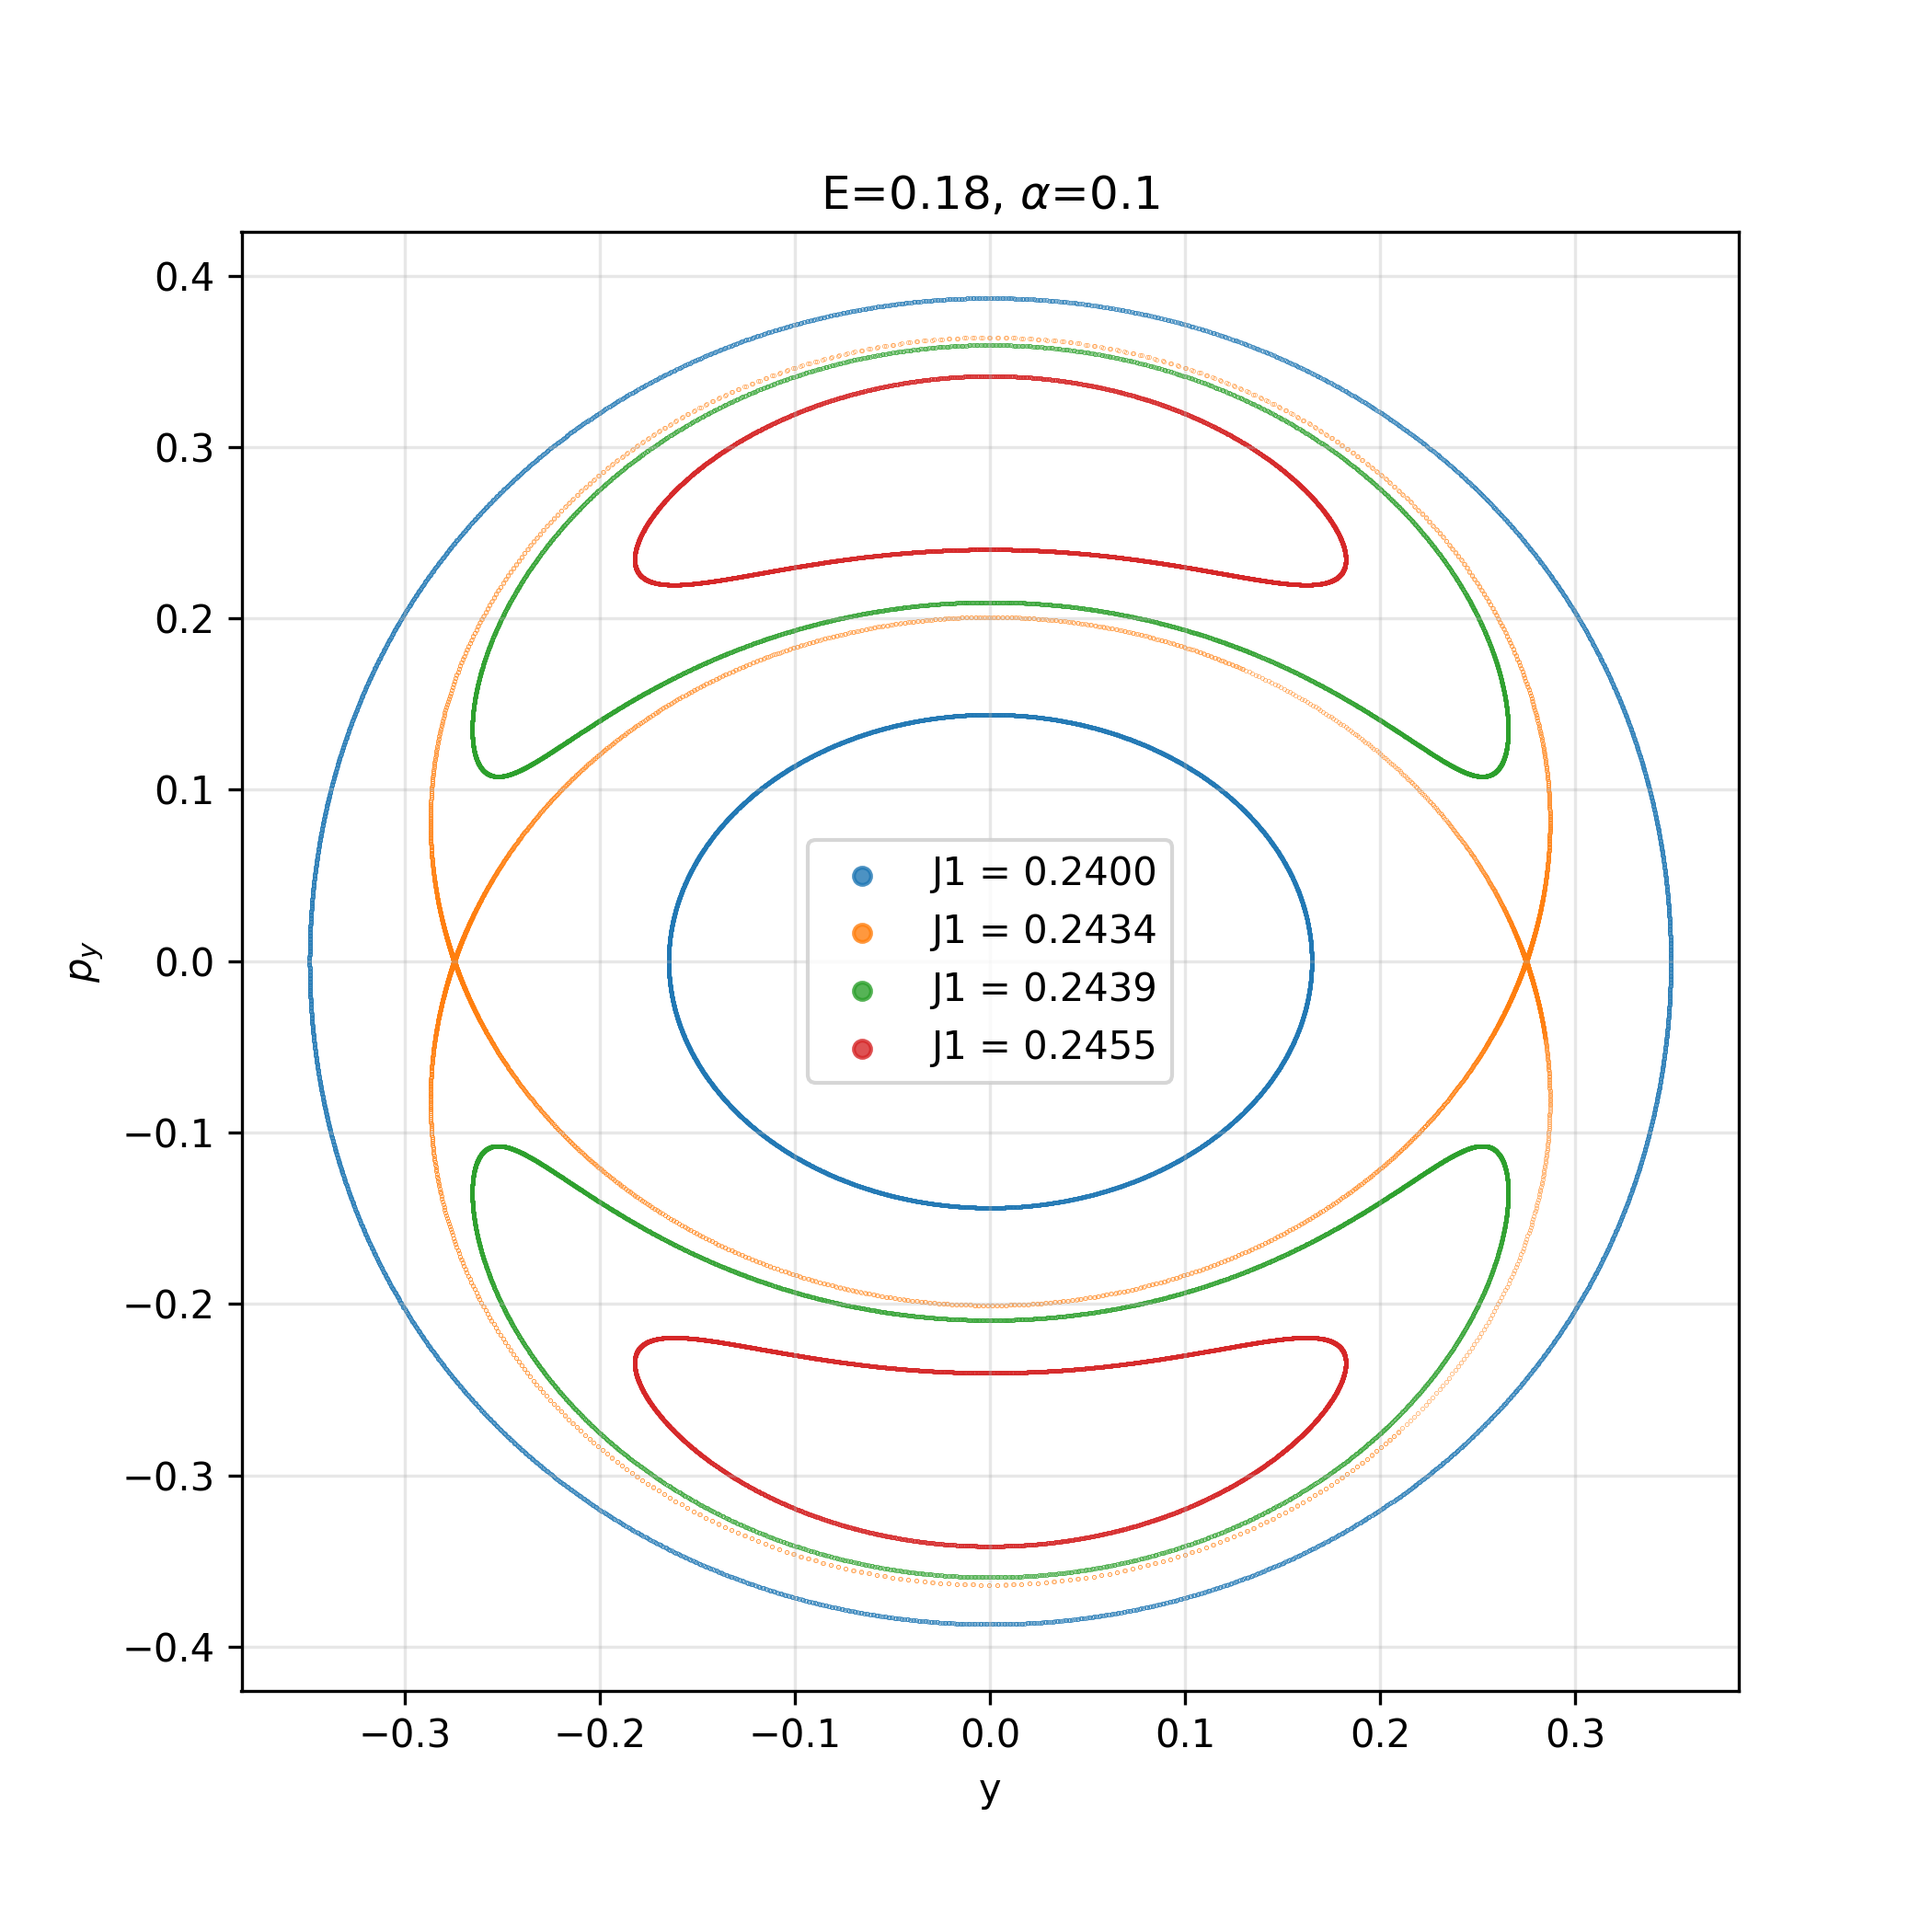
\includegraphics[width=0.5\textwidth]{figures/18_H22.png}
    \caption{\scriptsize Mappa di Poincare per il sistema bidimensionale di questa sezione, notiamo la risonanza in $J_1 = 0.24$. Per $\alpha\ll 1$ si dovrebbe avere la risonanza a $I_1\simeq 5I_2$. Numericamente questa non è esattamente rispettata, probabilmente $\alpha=0.1$ non basta.}
    \label{fig:figures-18_H22-png}
\end{figure}
\subsection{Sistema di Henon e Heiles: sono stabili le stelle delle galassie?}%
\label{sub:Sistema di Henon e Heiles}
Nel 1964 era noto che, il moto di una stella nella galassia presentava due integrali del moto: l'energia ed una componente del momento angolare.\\
Analiticamente nessuno riusciva a capire se fosse presente un altro integrale del moto, tuttavia le osservazioni del rapporto tra la velocità parallela al centro della galassia e quella ortogonale ne suggerivano la presenza (tale rapporto risultava circa 2:1).\\
Henon e Heiles ci riuscirono nell'intento modellizzando con una semplice Hamiltoniana:
\[
    H = \frac{1}{2}(p_x^2+p_y^2) + \frac{1}{2}(x^2+y^2) + x^2y-\frac{1}{3}y^3
.\] 
Quello che fecero è studiare la mappa: se si fosse presentata una terza costante del moto sarebbe apparsa nel numero di tori invarianti del sistema.
\begin{figure}[H]
    \centering
    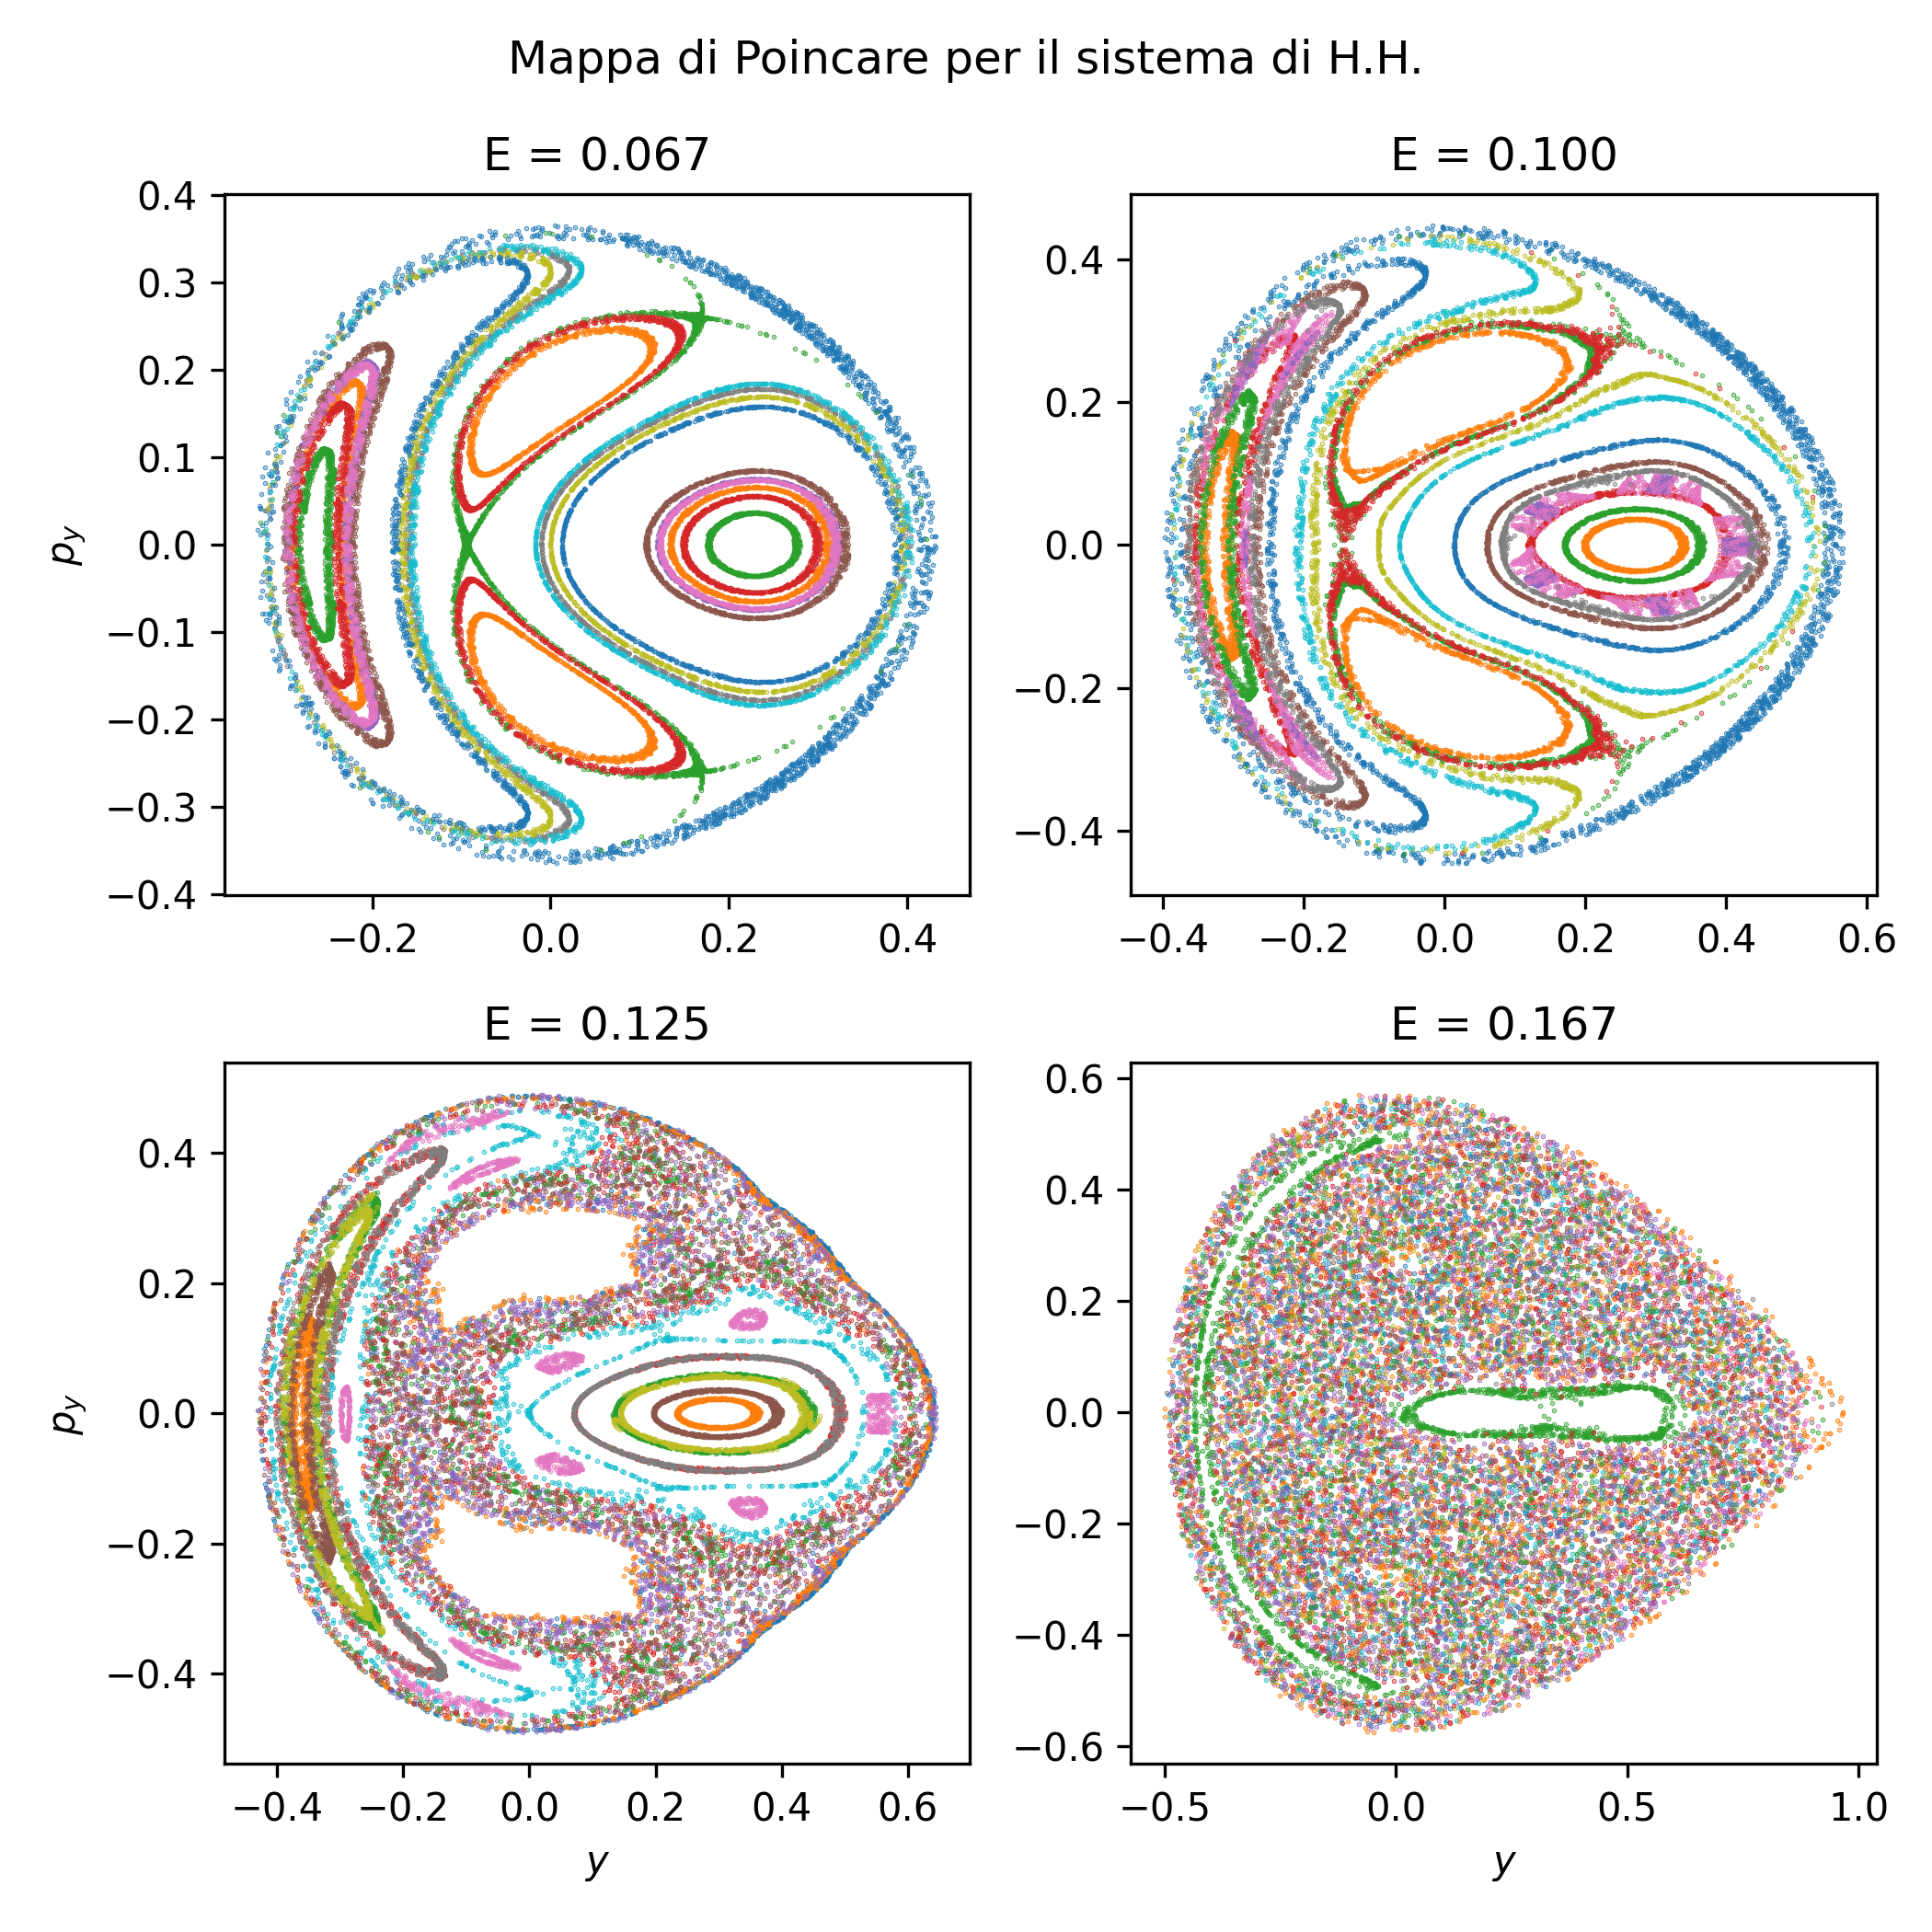
\includegraphics[width=0.45\textwidth]{figures/18_Henon-Heiles.png}
    \caption{\scriptsize Mappa di Poincare per il sistema di Henon-Heiles: notiamo come a bassa energia è evidente la presenza di tori invarianti: c'è un terzo integrale del moto.}
    \label{fig:}
\end{figure}
\noindent
Si vede bene che, all'aumentare della energia, i tori invarianti si rompono. In particolare si ha che i primi tori a rompersi sono proprio quelli passanti per il punto fisso: quelli corrispondenti a delle frequenze di H tra loro razionali.
\subsubsection{Tentativo di costruire una teoria perturbativa per Henon-Heiles}%
\label{subsub:Tentativo di costruire una teoria perturbativa per Henon-Heiles}
Il motivo per il quale non è stato possibile trovare un terzo integrale del moto analiticamente è il fallimento della teoria perturbativa. Andiamo in variabili azione-angolo:
\[
    \frac{1}{2}p_x^2 + \frac{1}{2}x^2 = \omega_xI_x
.\] 
\[
    \frac{1}{2}p_y^2 + \frac{1}{2}y^2 = \omega_yI_y
.\] 
Le trasformazioni canoniche associate sono:
\[\begin{aligned}
    x = \sqrt{2I_x} \sin\theta_x \qquad y = \sqrt{2I_y} \sin\theta_y
.\end{aligned}\]
In conclusione possiamo scrivere l'Hamiltoniana imperturbata come:
\[
    H_0 = \omega_xI_x + \omega_yI_y
.\] 
Mentre la perturbazione:
\[\begin{aligned}
    H_I = &\frac{(2I_x)(2I_y)^{1 /2}}{2}\times\\ 
	  &\times \left[\sin \theta_y-\frac{1}{2}\sin (\theta_x+\theta_y)-\frac{1}{2}\sin (\theta_x-2\theta_x) \right] + \\
	  & - \frac{1}{3}\left(2I_y\right)^{3 /2}\left[\frac{3}{2}\sin\theta_y-\frac{1}{2}\sin (3\theta_y)\right]
.\end{aligned}\]
In conclusione si dovrebbe trovare la trasformazione che integra la seguente H:
\[
    H = H_0+H_I
.\] 
Il grosso problema è che possiamo trovarne una che elimini una delle due risonanze in $\theta_y\pm 2\theta_x$
\footnote{Il problema di questi termini deriva dalla \textbf{interazione} delle due variabili angolo: tale interazione potrebbe distruggere la teoria perturbativa per la scelta di determinati valori iniziali ad esempio.}
, non è tuttavia possibile eliminarle entrambe. La teoria perturbativa quindi fallisce in questo caso e vediamo i tori nello spazio delle fasi rompersi all'aumentare dell'energia.\\
Nel seguito ci focalizzeremo su delle mappe che siano "\textbf{Area preserving}", ovvero quelle che derivano da sistemi Hamiltoniani.\\
Una mappa, per essere area preserving deve avere uno Jacobiano unitario, in due dimensioni ad esempio dovrà essere:
\[
    \frac{\partial (x_{i+1}, y_{i+1})}{\partial (x_i, y_i)} = 1
.\] 
La logica di questo cambio di punto di vista è la seguente: se studiamo degli insiemi generici di mappe (Area preserving) allora dato un qualunque sistema Hamiltoniano potremmo pensare di ricondurlo ad una determinate classi di mappe. \\
Questo approccio ci permette di risolvere generalizzando molti più problemi Hamiloniani.
\subsection{Twist Map}%
\label{sub:Twist Map}
Supponiamo di avere un toro bidimensionale avente frequenze tra di loro incommensurabili (rapporto irrazionale). Supponiamo inoltre che le due frequenze $\omega_1, \omega_2$ varino debolmente con l'azione $I$.\\
Dalla definizione di variabili azione angolo sappiamo che:
\[
    \theta_1(t)=\omega_1t+\theta_1(0) \qquad
    \theta_2(t)=\omega_2t+\theta_2(0)
.\] 
E anche:
\[
    \omega_1 = \partial_{I_1}H \qquad \omega_2 = \partial_{I_2}H
.\] 
Sia $t_2$  il periodo per avere $\theta_2\to \theta_2+2\pi$, sempre per definizione di pulsazione $\omega$ si ha:
\[
    t_2 =  \frac{2\pi}{\omega_2}
.\] 
Cosa possiamo dire sulla traslazione temporale di $t_2$  per $\theta_1$?
\[\begin{aligned}
    \theta_1(t+t_2) =& \theta_1(t)+\omega_1t_1 = \\
		     & = \theta_1(t) + 2\pi\frac{\omega_1}{\omega_2} = \\
		     & =\theta_1(t) + 2\pi  \frac{\omega_1}{\omega_2}(I_1)
.\end{aligned}\]
Attenzione al fatto che $\omega_1/\omega_2$ è una funzione di variabile $I_1$ (non è una moltiplicazione).\\
Operativamente una twist map ha una struttura sulla superficie di Poincare del seguente tipo:
\begin{redbox}{Twist map}
    \[
	x_i \equiv \left(\theta_1(t+it_2), I_1\right) \equiv (\theta_i, r_i)
    .\] 
    in cui la dipendenza da $r_i$ compare nel fattore $\omega_1 /\omega_2 \equiv \alpha (r_i)$.
\end{redbox}
\noindent
\begin{exmp}[Twist map semplice]
    \[
        \begin{cases}
	    \theta_{i+1} = \theta_i + 2\pi\alpha (r_i)\\
	    r_{i+1}=r_i
        \end{cases}
    .\] 
    Possiamo visualizzare la mappa nello spazio $x, y$:
    \[
	x_i = r_i\cos (\theta_i) \qquad y_i = r_i\sin (\theta_i)
    .\] 
    \[
        r = \sqrt{x^2+y^2} 
    .\] 
    In queste coordinate si ha che, se $\alpha$ non dipende da $r$, iterando la mappa i punti $x, y$ giacciono tutti sulla stessa circonferenza.
    Visto che in generale abbiamo una dipendenza da $\alpha$ allora i punti con $r$ maggiore ruotano di più o di meno rispetto a quelli con $r$ minore, formando quindi una specie di rotazione-dilatazione dello spazio ($x, y$).
    \begin{figure}[H]
        \centering
	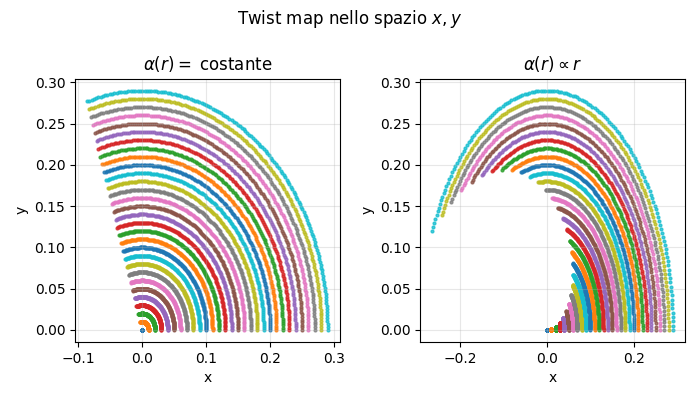
\includegraphics[width=0.45\textwidth]{figures/18_twist_tetha_r.png}
	\caption{\scriptsize Twist map nello spazio $x, y$, le condizioni iniziali utilizzate sono $\theta_0 = 0$. Per $r_0$ sono stati selezionati diversi valori tra $0$ e $0.3$ che danno origine alle curve rotanti (un colore corrisponde alla singola traiettoria, dopo il celeste la mappa di colori si ripete).}
        \label{fig:-figures-18_twist_tetha_r-png}
    \end{figure}
\end{exmp}
\noindent
\begin{exmp}[Twist map in cartesiane]
    Un esempio di Twist map in coordinate cartesiane è:
    \[
        \begin{cases}
            x_{i+1}=x_i+y_i\\
	    y_{i+1}=y_i
        \end{cases}
    \] 
    Notiamo che la struttura delle equazioni è identica al caso precedente (in coordinate polari).\\
    Questa mappa è area preserving, infatti:
    \[
        \begin{pmatrix} x_{i+1} \\ y_{i+1} \end{pmatrix} =
	\begin{pmatrix} 
	    1 & 1 \\
	    0 & 1
	\end{pmatrix} 
	\begin{pmatrix} x_i \\ y_i \end{pmatrix} 
    .\] 
    Partendo con dei punti aventi tutti la stessa coordinata $x$ si osserva che, per iterate successive, i punti con la $y$ maggiore vengono mandati in $x$ maggiori rispetto a quelli con una $x$ minore. La coordinata $y$ resta invece inalterata.\\
    Abbiamo quindi una rotazione $+$ dilatazione nello spazio $x,y$: una Twist map.
\end{exmp}
\noindent
\clearpage
